\documentclass{article}
\usepackage[utf8]{inputenc}
\usepackage{float}
\usepackage{xcolor}
\usepackage{graphicx}
\usepackage{amsmath}
\usepackage{amssymb}
\usepackage{placeins}

\usepackage{hyperref}
\hypersetup{
    colorlinks=true,
    linkcolor=blue,
    filecolor=magenta,      
    urlcolor=blue,
}

\title{Scientific Computing - Molecular dynamics \\ Group F}
\newcommand{\subtitle}{Problem sheet 3}
\author{
    Jimin Kim \\
    Christian Nix \\
    Noah Schlenker
}
\date{\today}

\begin{document}

\maketitle

\begin{center}
    \LARGE \subtitle{}
\end{center}

\section{Pull request}
\label{sec:pr}
The pull request can be found \href{https://github.com/noahpy/MolSim-SS24/pull/33}{here}.

\section{XML format adaptation}
\label{sec:xml}

\begin{itemize}
    \item We defined the structure and constraints for XML files using XSD .
    \item The key elements specified include:
    \begin{itemize}
        \item Standard parameters as outlined in Task 1, such as base name and cuboid specification etc.
        \item Domain specifications and cutoff-radius
        \item Boundary condition specifications
    \end{itemize}
    \item We utilized several flags in the XSD CMake module:
    \begin{itemize}
        \item \texttt{cxx-tree}: Converts XML documents to a tree-like in-memory object model, generating corresponding C++ classes.
        \item \texttt{--hxx-suffix=.h} and \texttt{--cxx-suffix=.cpp}: Specifies suffixes for the generated header and source files.
        \item \texttt{--std=c++11}: Ensures the generated C++ code adheres to the C++11 standard.
        \item \texttt{--generate-doxygen}: Adds Doxygen comments to the generated code.
        \item \texttt{--generate-serialization}: Includes serialization support, allowing XML data to be read from and written to XML documents.
    \end{itemize}
\end{itemize}

\section{Linked-Cell Algorithm}
\label{sec:lc}

\begin{itemize}
    \item We added the cell and cell-grid to the models to implement the linked-cell algorithm (see \texttt{src/models/linked\_cell}).
    \item A new simulation class \texttt{linkedLennardJonesSim} and force calculation function \texttt{force\_lennard\_jones\_lc} were introduced for using linked-cells in our project structure (see \texttt{src/simulation} and \texttt{src/physics/forceCal}).
    \item Each added section has its corresponding Unit tests.
\end{itemize}

\subsection{Cells}
\label{subsec:cell}

\begin{itemize}
    \item Each cell contains a list of references to particles and a \texttt{type} attribute, categorized as \texttt{inner}, \texttt{boundary}, or \texttt{halo}.
    \item The \texttt{CellIndex} and \texttt{neighborCounter} attributes are essential for the cell-grid structure.
    \item Neighbor vectors include information on the index and position of boundary, inner, and halo neighbors within the grid.
    \item A \texttt{PairListIterator} enables iteration over unique pairs in the reference list.
\end{itemize}

\subsection{Cell Grid}
\label{subsec:grid}

\begin{itemize}
    \item Our cell grid is implemented using a 3-dimensional vector matrix, \texttt{CellVec}, which contains \texttt{std::unique\_ptr} to cells.
    \item Initialization requires \texttt{domainSize}, \texttt{domainOrigin}, and \texttt{cutoffRadius}, and performs the correct cell type selection.
    \item The initialization function ensures uniform and fitting cell sizes.
    \item Particle references in each cell's list are assigned from the existing particle container's vector.
    \item This file includes most necessary functions for running a simulation and calculating forces using the linked-cell algorithm.
    \item Noteworthy is the function \texttt{std::list<CellIndex> getNeighbourCells(const CellIndex\& cellIndex) const}, which returns a list of neighboring cell indices for a given cell:
    \begin{itemize}
        \item It checks if the \texttt{visited} boolean of parameter cell is false. If not visited, it stores the particle forces to the old forces and zeros them.
        \item It iterates over each neighboring cell and increments \texttt{neighborCounter} for each non-halo neighbor.
        \item If a neighboring cell's \texttt{neighborCounter} > 0, the counter is decreased, and the neighbor is ignored. If the counter reaches zero, the visited status is reset.
        \item Otherwise, the neighbor's index is added to the return list.
        \item If the neighbor hasn't been visited, the status is set to visited, and the particle forces are prepared for calculations.
    \end{itemize}
    \item We implemented the iterators for halo and boundary cells in a separate file for clarity.
\end{itemize}

\subsection{Performance test}
\label{subsec:perflc}

\begin{itemize}
    \item We added a benchmark test for the linked-cell implementation \newline(see \texttt{bench/benchLinkedCell.cpp}).
    \item We tested the performance of with the parameters stated in Task 2 \newline(see\ \ref{fig:timelc} and\ \ref{fig:timelclong}).
    \item The hardware specifics for running the tests are shown here\ \ref{fig:specs}.
\end{itemize}

\FloatBarrier

\begin{figure}[H]
    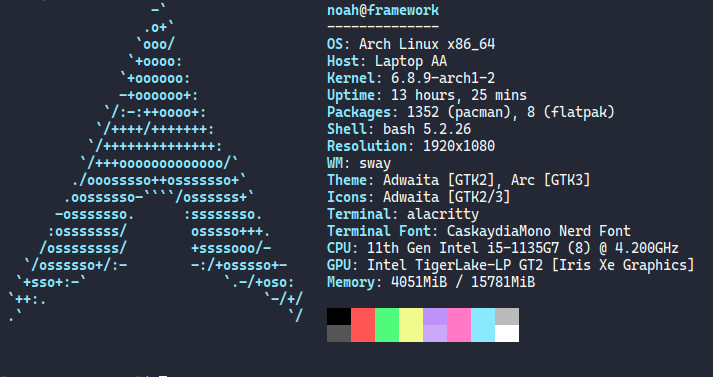
\includegraphics[width=\textwidth]{res/neofetch}
    \caption{Hardware specifications for the performance tests.}
    \label{fig:specs}
\end{figure}

\begin{figure}[H]
    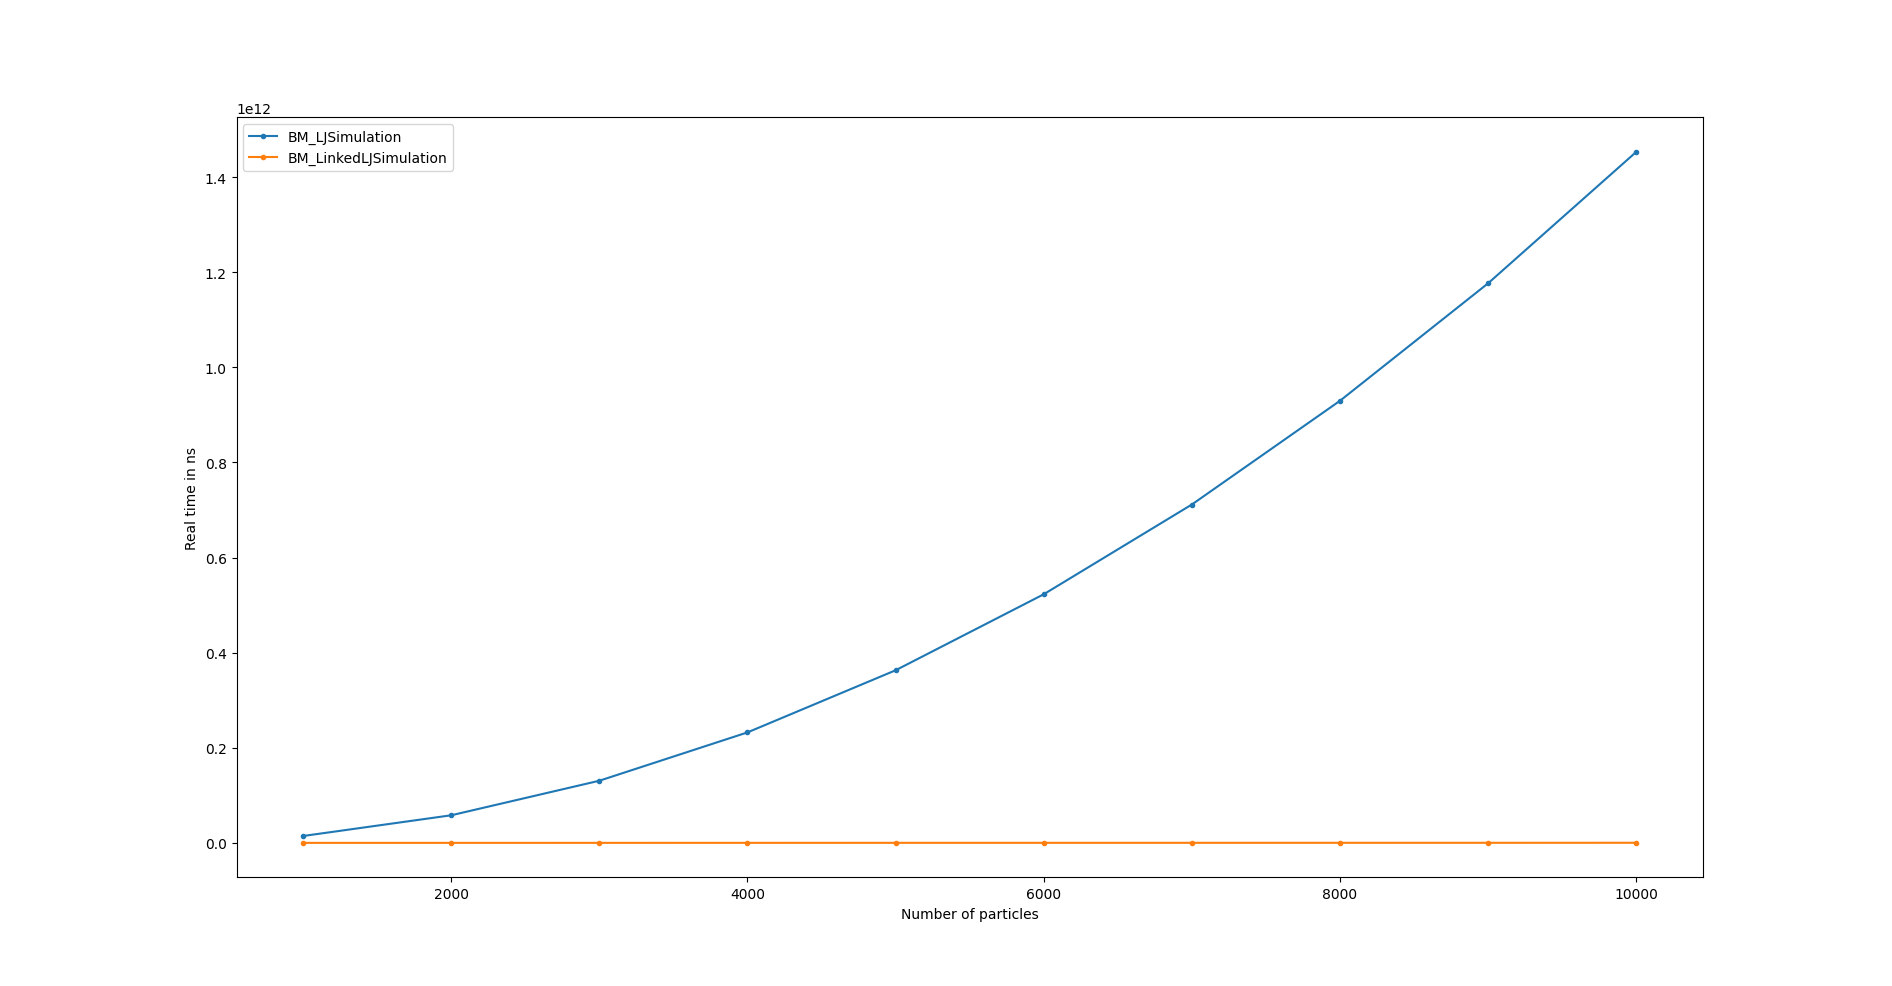
\includegraphics[width=\textwidth]{res/lj_big_plot_linear}
    \caption{linked-cell and naive simulation times of a 2D-square with 1000 to 10000 molecules.}
    \label{fig:timelc}
\end{figure}

\begin{figure}[H]
    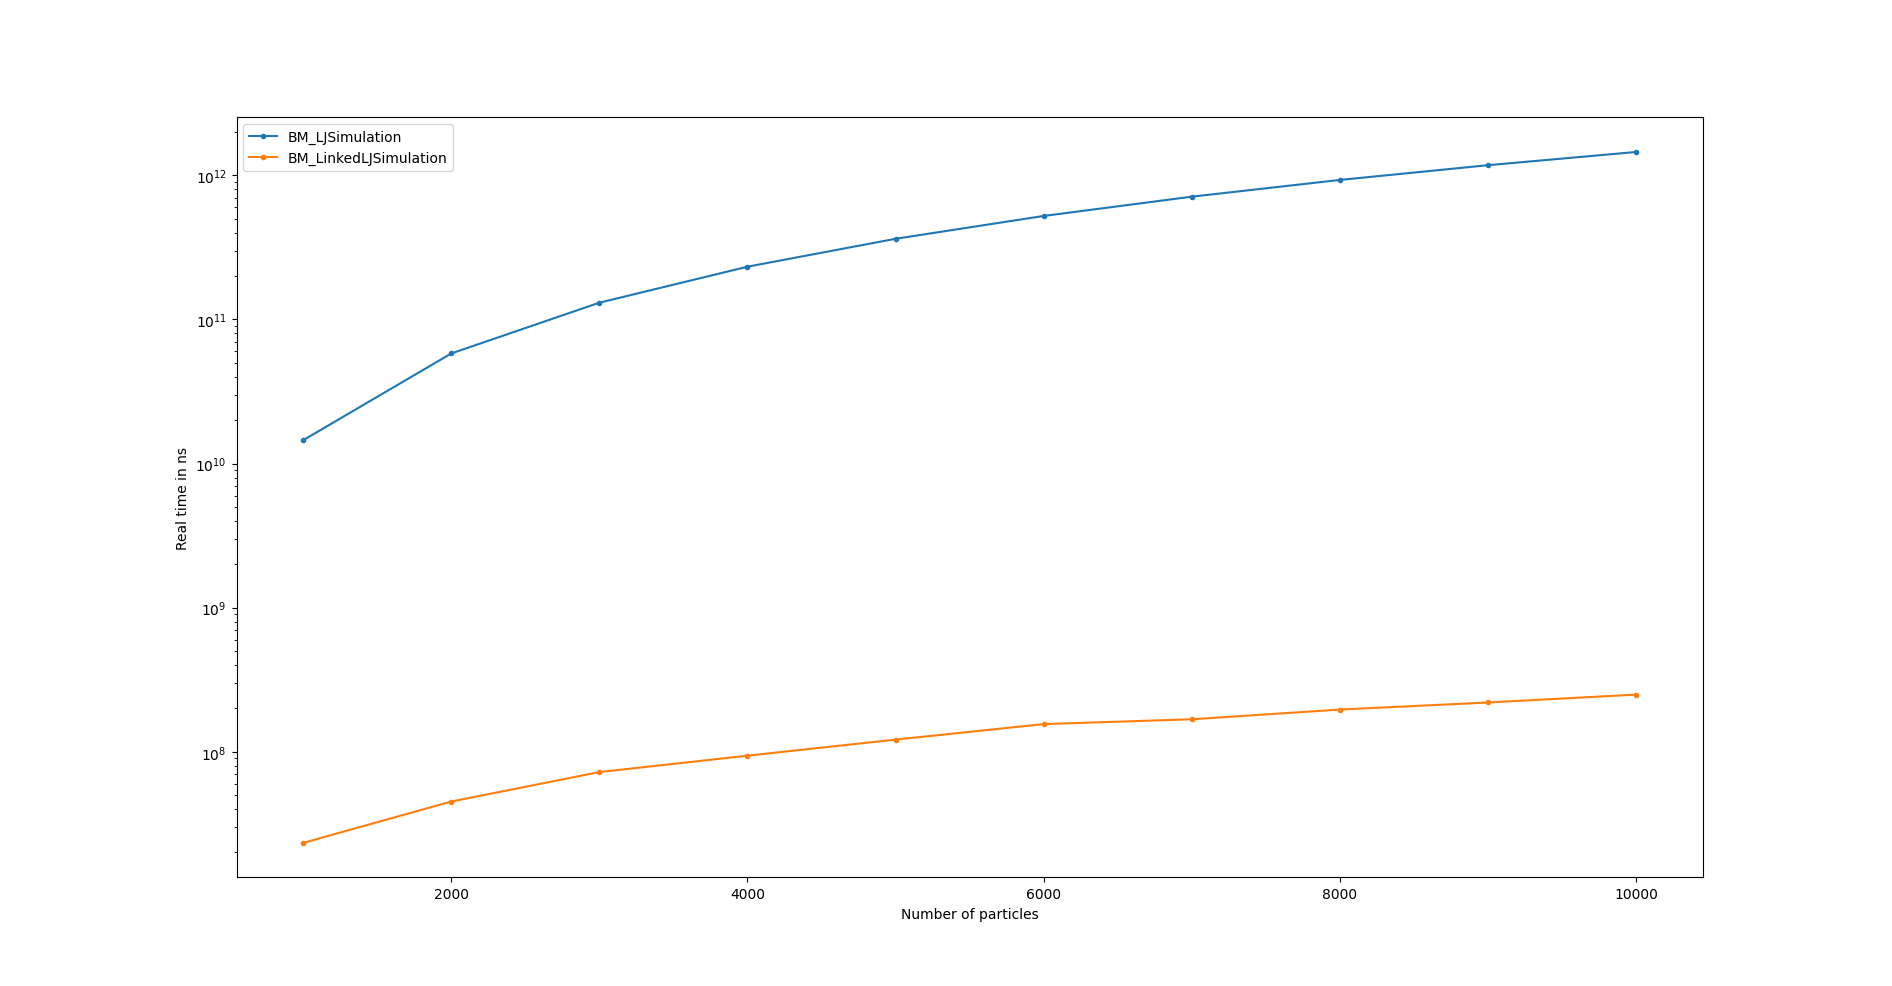
\includegraphics[width=\textwidth]{res/lj_big_plot_log}
    \caption{linked-cell and naive simulation times with 1000 to 10000 particles and a logarithmic time scale}
    \label{fig:timelclong}
\end{figure}

\section{Boundary Conditions}
\label{sec:bound}

\begin{itemize}
    \item We added boundary conditions to the physics section of our project (see \texttt{src/physics/boundaryConditions}).
    \item A Handler organizes the conditions for each boundary in a simulation specified in the boundary configuration file.
    \item The boundary condition is a virtual class, and provides functions for applying the conditions before and after updates in the cell grid.
    \item We have two implementations of boundary conditions as described in the third meeting:
    \begin{itemize}
        \item \texttt{OverflowBoundary}: Particles are removed if they leave the domain.
        \item \texttt{SoftReflectiveBoundary}: Particles are reflected from the boundaries via a mirrored ghost particle in the neighboring halo cell. This required an additional function to find the relevant halo cell for creating the ghost particle.
    \end{itemize}
\end{itemize}

\section{Sphere generation}
\label{sec:sphere}

\begin{itemize}
    \item We extended the particle generators with a class to generate sphere clusters (see \texttt{src/models/generators/SphereParticleCluster})
    \item The logic of sphere generation can be split into 2D and 3D:
    \begin{itemize}
        \item 2D Discs: The disc is created as a collection of concentric rings of particles. \texttt{generateRing()} creates a ring of particles evenly spaced around a circumference and \texttt{generateDisc()} generates rings of particles with decreasing radii.
        \item 3D Sphere: The sphere is constructed as a stack of discs. Discs above and below the origin are iteratively generated with decreasing radii.
    \end{itemize}
    \item Even spacing of particles in rings is achieved through the use of several trigonometric functions:
    \begin{enumerate}
        \item Angular step calculation:
        \begin{itemize}
            \item We calculate the angular step $\theta$ between particles to ensure they are spaced by at least a given distance along the circumference.
            \item Given a ring with radius \textit{r} and particle spacing \textit{s}, the angular step $\theta$ is determined by:
            \item $\theta = 2 \arcsin\left(\frac{s}{2 \times r}\right)$
        \end{itemize}
        \item Number of particles calculation:
        \begin{itemize}
            \item The number of particles \textit{N} that can fit in the ring is given by dividing the full circle ($2\pi\ radians$) by the angular step $\theta$:
            \item $N = \left\lfloor \frac{2\pi}{\theta} \right\rfloor$
        \end{itemize}
        \item Positioning particles:
        \begin{itemize}
            \item The coordinates for each particle in the ring are calculated using polar coordinates.
            \item For a particle at index \textit{i}, the position is:
            \item $x_i = \text{origin}_x + r \cos(i \theta)\newline y_i = \text{origin}_y + r \sin(i \theta)\newline z_i = \text{origin}_z + \text{z\_offset}$
        \end{itemize}
    \end{enumerate}
\end{itemize}

\end{document}
